%!TEX root = ../report.tex
\chapter{Software Development Method}\label{chap:sw_dev_method}
One of the great challenges this semester is to coordinate the development process across all 15 groups. This chapter defines the development method as it looks at the end of the project.

\begin{chapterorganization}
  \item in \sectionref{sec:project_overview} we describe how the multi-project is organized and introduce the hierarchy of the project;
  \item in \sectionref{sec:swmethod_ourgroup} we describe the software development method in our group;
  \item in \sectionref{sec:multi_project_group_roles} we detail the responsibilities delegated to specific groups.
\end{chapterorganization}

\begin{abbreviations}
  \item[\gui] Graphical User Interface
  \item[\db] Database
  \item[\bd] Build \& Deployment
  \item[PO] Product Owner
\end{abbreviations}

\section{Multi-Project Organization Method}\label{sec:project_overview}
The multi-project consists of 15 groups. All groups collaborate on building the Giraf applications. The groups are organized into three subprojects: \emph{Graphical user interface} (\gui), \emph{databases} (\db), and \emph{build and deployment} (\bd) by recommendation of the semester coordinator.

The \gui groups deal with bugs and implement new features in the front-end apps. The \db groups manage and maintain the database. The \bd groups control the tools supporting the building and testing environment as well as the deployment of the apps.

The multi-project groups work with an iterative development method, and the semester is divided into four iterations. No groups have any prior experience with the code base at the start of the project, nor with the requirements of the external customers. Therefore there are many uncertainties associated with the multi-project. This makes the application of an agile method suited for the project. Suppose the multi-project is organized in a traditional method. Then the multi-project groups will spend much time initially analyzing the current code base and future requirements, rather than actually work on making the code base work (a prime wish of the external customer). These requirements may change over time, which makes it difficult to deliver what the users want.

The agile method used for the project is Scrum, and the groups are organized as Scrum of Scrums. Scrum of Scrums divides the developers into several layers of Scrum teams \parencite{scrum_of_scrums2015}. \figureref{fig:multi_project_organization} shows the structure of the multi-project organization, which consists of three levels:

\begin{description}
  \item[Multi-Project Level] The purpose of the overall level is to ensure that the roles, work products, and meetings are followed as intended. That is, that the development method is followed. A weekly meeting is held where the status of each subproject is discussed, and the development method and roles are evaluated. Every group has at least one representative at the weekly multi-project meetings.
  \item[Subproject Level] Each subproject has the responsibility of solving a number of backlog items related to either \gui, \db, or \bd. Representatives from each group in a subproject have sprint planning and sprint review meetings with the other members of the subproject and hold at minimum two Scrum meetings a week. We choose not to meet every day because we think that it will steal too much time, compared to the benefits. It is common for such a meeting to be held two or three times a week \parencite{scrum_of_scrums2015}.
  \item[Group Level] Each group solves some of the backlog items of its subproject. While Scrum of Scrums dictates that Scrum is followed at all levels, this is not the case for this multi-project organization. This is of course a major deviation from Scrum of Scrums. When initially deciding the software development method, some groups expressed an interest in not running Scrum. Thus, each group is given the freedom to organize how they see fit. However, all groups are expected to fill in the work products and attend the meetings described later.
\end{description}

\begin{figure}%
\centering
\tikzsetnextfilename{multiproject_illustration}
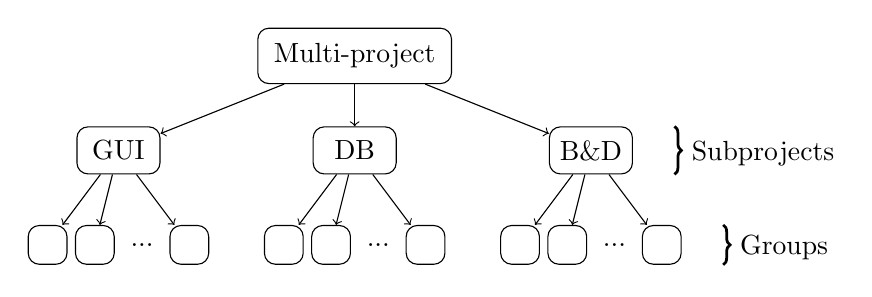
\begin{tikzpicture}[
  simple/.style={draw, rounded corners, minimum height=2em, minimum width=7em},
  simplefixed/.style={draw, rounded corners, minimum height=1.7em, minimum width=3em},
  square/.style={draw, rounded corners, minimum height=1.4em, minimum width=1.4em}]

  \node[simple] (mp) at (0,0) {Multi-project};

  \node[simplefixed] (gui) at (0,-1.2) {DB}; % NOTICE OTHER NAME THAN LABEL.
  \node[simplefixed] (db) at (-3,-1.2) {GUI};
  \node[simplefixed] (bd) at (3,-1.2) {B\&D};

  \node[square] (g1) at (-3.9, -2.4) {};
  \node[square] (g2) at (-3.3, -2.4) {};
  \node[] (g3) at (-2.7, -2.4) {...};
  \node[square] (g4) at (-2.1, -2.4) {};

  \node[square] (g5) at (-0.9, -2.4) {};
  \node[square] (g6) at (-0.3, -2.4) {};
  \node[] (g7) at (0.3, -2.4) {...};
  \node[square] (g8) at (0.9, -2.4) {};

  \node[square] (g9) at (2.1, -2.4) {};
  \node[square] (g10) at (2.7, -2.4) {};
  \node[] (g11) at (3.3, -2.4) {...};
  \node[square] (g12) at (3.9, -2.4) {};

  \draw[->] (mp) to (gui);
  \draw[->] (mp) to (db);
  \draw[->] (mp) to (bd);

  \draw[->] (db) to (g1);
  \draw[->] (db) to (g2);
  \draw[->] (db) to (g4);

  \draw[->] (gui) to (g5);
  \draw[->] (gui) to (g6);
  \draw[->] (gui) to (g8);

  \draw[->] (bd) to (g9);
  \draw[->] (bd) to (g10);
  \draw[->] (bd) to (g12);

  \draw[decorate, line width=1pt, decoration={brace, mirror}] ([xshift=1.5em]g12.south east) -- ([xshift=1.5em]g12.north east) node [midway, yshift=-0.1em, xshift=2.2em] {Groups};

  \draw[decorate, line width=1pt, decoration={brace, mirror}] ([xshift=1.5em]bd.south east) -- ([xshift=1.5em]bd.north east) node [midway, yshift=-0.1em, xshift=3.2em] {Subprojects};

\end{tikzpicture}
\caption{Illustration of multi-project organization}%
\label{fig:multi_project_organization}%
\end{figure}

\subsection{Work Products}
Two work products from Scrum are used, and every group is expected to help updating and maintaining these:

\begin{description}
  \item[Product Backlog] The product backlog contains the items of value to the customers, typically features, but also other items \parencite{larman2003}. On the multi-project level, there is a product backlog containing all items for the entire multi-project. The purpose of the multi-project level product backlog is to maintain the product backlog for the entire multi-project. The items in the product backlog are categorized according to each subproject. This enables each subproject to manage their items themselves, removing unnecessary management from the multi-project level.
  \item[Release Backlog] The release backlog contains the items that must be finished by the end of the current sprint \parencite{larman2003}. These items are selected from the product backlog during sprint planning meetings that each subproject hold.
\end{description}

Since it is not required for each group to use Scrum at the group level, there is no common sprint backlog.

The product backlog and release backlog contain the following items:

\begin{description}
  \item[Feature] Functional requirements (features) of the product are represented as user stories, as they are lightweight and fit well into the agile principles \parencite{rubin2012essential}.
  \item[Bug] Because bugs also represents behavior the user wants to be changed, they are considered no different from features \parencite{product-backlog2015}, and so are represented as user stories.
  \item[Constraint] A way of handling non-functional requirements, while not forcing it into a user story, is to turn the non-functional requirements into constraints \parencite[ch.16]{cohn2004}. Most often, these constraints are related to e.g.\ performance, usability, and security. Constraints can either be written on separate constraint cards \parencite[ch.16]{cohn2004}, or written in the corner of a user story card if it is relevant only to that single user story \parencite[ch.7]{cohn2004}. Due to the structure of multi-project, it makes sense for us to introduce two-level constraints. Multi-project constraints are relevant for the entire project as a whole, for example \emph{the software is written in Java} or \emph{all apps must be easy to internationalize}. Some constraints only apply to some areas of the project, and these are handled by the individual groups. Examples of these are \emph{the initial database sync must not take more than 5 minutes} or \emph{the user manager must only sync data of the user logged in}. These constraints are written on either a constraint card or on the relevant backlog item.
  \item[Knowledge Acquisition] Since no one in the multi-project has worked on it before, and because the project is complex, it is sometimes needed to investigate things to know it if is worth investing time in. Knowledge acquisition items can be formulated as user stories, but do not need to \cite{rubin2012essential}. Knowledge acquisition items are handled the same way as user stories. Estimation can be hard when investigating an unknown subject. The item can be investigated just enough to do further estimation by \emph{timeboxing} an initial investigation. This practice is in XP called a \emph{spike} \cite{cohn2004}.
  \item[Technical Work] Sometimes effort has to be spent on something the users are not directly interested in, e.g.\ updating software on the developer machines, updating the database software on a server, or refactoring parts of the code. These items can be part of the product backlog \cite{cohn2004}. They can also be formulated the same way as user stories \cite{rubin2012essential} and are handled the same way.
\end{description}

To summarize, the backlog items \emph{features} and \emph{bugs} are represented as user stories, whereas \emph{knowledge acquisition} and \emph{technical work} can be represented as user stories, but do not need to.

The following template, presented by \textcite{cohn2009}, is used for user stories in the multi-project:

$$\text{As a $\langle{}$\emph{type of user}$\rangle{}$, I want $\langle{}$\emph{some goal}$\rangle{}$ so that $\langle{}$\emph{some reason}$\rangle{}$}.$$

If the user story is suggested by developer, the source of the user story should be noted in case there are questions about it.

A user story must be sufficiently small for it to be completed in one sprint \parencite{cohn2009}. A user story must also have \emph{conditions of satisfaction}. These are high-level acceptance tests for the user story and must be true for the user story to be completed. A user story can have multiple conditions of satisfaction \cite{cohn2009}. Backlog items are prioritized by the product owner (possibly with help from the customers) \cite{larman2003}.

\todo{indsæt eksempel på US + SAT}

\subsection{Roles}
Two roles from Scrum are used in the multi-project:

\begin{description}
  \item[Scrum Master] \todo{Read this, it is revised} On the multi-project level, we are responsible for the development method. This means that we act as Scrum masters on the multi-project level. It is our role as Scrum masters to know and reinforce the sprint and project goals and visions and to ensure that the Scrum practices and values are followed on the multi-project level \cite{larman2003}. On the subproject level, one person is in charge of the meetings --- they make sure that the Scrum meetings on this level are held. On the group level, each group is free to do what they see fit.
  \item[Product Owner] The product owner (PO) is responsible for maintaining contact with the customers and being their representatives. It can be difficult to have a single PO with an external customer as customer in the multi-project. Therefore, the \bd and \db groups often do not have the external customer as their direct customer. Rather, these groups help the \gui groups achieve their goal by building solutions for them. The external customer is often not interested in the implementation details of build and database interfaces.

There are three POs in the multi-project, one for each subproject. The customer for the \gui PO is the external customer, whereas the customers for the \db and \bd POs are the groups of the other subprojects, as illustrated in \figureref{fig:po_illu}.
\end{description}

\begin{figure}%
\centering
\tikzsetnextfilename{po_illustration}
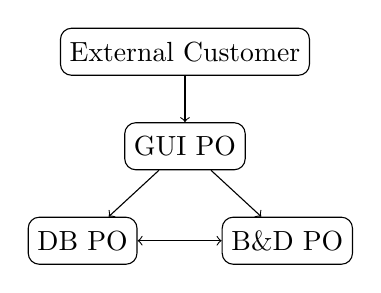
\begin{tikzpicture}[
  simple/.style={draw, rounded corners, minimum height=1.7em}]
  \node[simple] (extcust) at (0,1.2) {External Customer};
  \node[simple] (guipo) at (0,0) {GUI PO};
  \node[simple] (dbpo) at (-1.3,-1.2) {DB PO};
  \node[simple] (bdpo) at (1.3,-1.2) {B\&D PO};

  \draw[->] (guipo) to (dbpo);
  \draw[->] (guipo) to (bdpo);
  \draw[<->] (dbpo) to (bdpo);
  \draw[->] (extcust) to (guipo);

\end{tikzpicture}
\caption{Illustration of product owners}%
\label{fig:po_illu}%
\end{figure}

\subsection{Meetings}\label{sec:meetings}
Each week there is a meeting at the multi-project level. At this meeting the status of all groups in the multi-project is presented and the development method is evaluated. This ensures that all groups know the current status of the project. This meeting differs from a regular Scrum meeting in that it includes a point on method evaluation, so that the development method can be continually improved.

Each subproject holds internal Scrum meetings as well. These subproject Scrum meetings are held at least twice a week. The subprojects organize these meetings themselves and use them to discuss things that are relevant only for the members of the subproject.

Since there are three product owners in the multi-project, three sprint review meetings and three sprint planning meetings are held between sprints. These meetings were proposed by us, following the recommendation from \textcite{bird_davies_2007}, and afterward approved by the other groups.

\begin{description}
  \item[Sprint Planning Meetings]
  The purpose of the sprint planning meetings is to ensure that the product backlog is up to date and to select user stories for the release backlog.
  \begin{description}
    \item[GUI] At this sprint planning only one representative from each GUI group participate as \emph{pigs} (people who are allowed to talk), as well as the GUI PO and one representative from the other PO groups (although they have a less important role at this meeting). All other people in the multi-project are \emph{chickens} (people who are not allowed to talk). This meeting is held with the external customers. By making it so that primarily the \gui groups are pigs, the external customers are abstracted from internal development such as continuous integration and database management.
    \item[\db and \bd] There are separate sprint planning meetings for \db and \bd, where each subproject establishes the needs of the other subprojects. These meetings are internal, and the external customers do not participate, since \db and \bd do not have these as direct customers. \db and \bd will primarily have the GUI groups as their customers, who need various services from the \db and \bd subprojects, in order for them to fulfill their own backlog items directly related to the external customers. However, it might be that \db needs something from \bd and vice versa. Again, this abstracts the external customers from internal development.
  \end{description}
  \item[Sprint Review Meetings]
  At the sprint review meetings, the work done in the sprint is presented to the customers.
  \begin{description}
    \item[GUI] At this meeting the external customers are presented with the work of the GUI groups. Only the GUI groups participate as pigs at this meeting.
    \item[\db and \bd] \db and \bd each hold a separate sprint review meeting where they show the groups in the other subprojects what they have done in a sprint. The external customers are not present at these meetings, so that they are not bored with internal details. The \gui sprint planning meeting is separated from the \db and \bd sprint planning meeting by a few days, such that the product owners have time to organize, and make the requirements propagate from \gui to the other subprojects.
  \end{description}
  \item[Sprint Retrospective Meeting] \todo{Read this: this is new} The purpose of this meeting is to learn from the past to improve productivity in the future, a time for diagnosis of the multi-project \cite{scrumChecklist}. This meeting is held the Tuesday following a Sprint Review Meeting. In this meeting the previous sprint is discussed. There is extra focus on any problems regarding the process during this meeting. Any concerns that are raised during this meeting are discussed, and possible solutions are suggested.
\end{description}

The sprint timeline is shown in \figureref{fig:gantt_dates}. Each sprint has approximately 8 full days per man. The exact sprint meeting dates are as follows:
\begin{itemize}
  \item Sprint 1
  \begin{itemize}
    \item \gui{}, \db{}, and \bd{} sprint planning meetings: February 15
    \item \gui{}, \db{}, and \bd{} sprint review meetings: March 10
  \end{itemize}
  \item Sprint 2
  \begin{itemize}
    \item Sprint 2 \gui{}, \db{}, and \bd{} planning meetings: March 12
    \item Sprint 2 \gui{}, \db{}, and \bd{} review meetings: April 8
  \end{itemize}
  \item Sprint 3
  \begin{itemize}
    \item Sprint 3 \gui{} planning meeting: April 8
    \item Sprint 3 \db{} and \bd{} planning meetings: April 15
    \item Sprint 3 \gui{}, \db{}, and \bd{} review meetings: April 27
  \end{itemize}
  \item Sprint 4
  \begin{itemize}
    \item Sprint 4 \gui{} planning meeting: April 27
    \item Sprint 4 \db{} and \bd{} planning meetings: May 4
    \item Sprint 4 \gui{}, \db{}, and \bd{} review meetings: May 20
  \end{itemize}
\end{itemize}
Notice that the \gui{} sprint planning meetings in the first two sprints are not separated from the \db{} and \bd{} planning meetings, as this delay was introduced after sprint 2.

\begin{figure}[ht]
  \centering
  \tikzsetnextfilename{gantt_dates}
  \begin{tikzpicture}
    \begin{ganttchart}[x unit=1mm, time slot format=isodate]{2015-02-10}{2015-05-30}
      \gantttitlecalendar{month=name}\\
      \ganttgroup{Sprint 1}{2015-02-15}{2015-03-10}\\
      \ganttgroup{Sprint 2}{2015-03-12}{2015-04-08}\\
      \ganttgroup{Sprint 3}{2015-04-15}{2015-04-27}\\
      \ganttgroup{Sprint 4}{2015-05-04}{2015-05-20}\\
      \ganttmilestone[milestone left shift=-0.9, milestone right shift=1.9]{Project Deadline}{2015-05-27}
    \end{ganttchart}
  \end{tikzpicture}
  \caption{\label{fig:gantt_dates} Gantt chart illustrating the sprint timeline}
\end{figure}

\subsection{Office Hours}
A vital part of working agile involves being able to easily communicate with all members of the multi-project. To ensure this all groups must be reachable on e-mail all weekdays 09:00--15:00, and preferably be in the group rooms. An exception for this is when there are courses.

\subsection{Tools}\label{sec:tools}
To support the development method of the multi-project, an online project management tool, Redmine \parencite{redmine-website}, is used. This tool was in use the previous year, and so this year the multi-project continues to use it. The main features are:

\begin{description}
  \item[Wiki] A wiki is used for various information, such as guides, how the development method is structured, meeting minutes, etc. Previous years had several separate wikis for each subproject. This year there is a single wiki providing central information.
  \item[Forum] The forum is used for non-crucial communication. It is mostly used for non-work related discussions such as social events. Groups are encouraged to communicate to each other directly by going to each other's group rooms, rather than using the forum.
\end{description}

In addition to Redmine, Google Docs is used by the POs to maintain the backlog.

\section{Software Development Method in Our Group}\label{sec:swmethod_ourgroup}
In our group we use Scrum as the development method, because it fits well into the multi-project development method. We have a Daily Scrum each morning where we summarize our work since last time and what we intend to do until the next Daily Scrum.

In addition to the previously described work products, we use a sprint backlog. After a sprint planning where backlog items have been selected by each group, we then split the backlog items selected by us into tasks and estimate those tasks using planning poker. Our unit of estimation is in half days, with the smallest unit being 1. This means that tasks that can actually be completed in less than a half day, may become overestimated. However, since there is an inherent imprecision in our estimations, this is not an issue. Our sprint backlog is physically placed on a wall, so that we can easily manage our tasks. In addition to the sprint backlog we use a burndown chart to measure our progress.

\todo{insert picture of wall}

\section{Group Roles in Multi-Project}\label{sec:multi_project_group_roles}
The multi-project contains responsibilities selected by groups within the multi-project. These roles include management of Redmine, server, Git, and Jenkins:

\begin{description}
  \item[Redmine General] Maintaining users, roles, and plugins on Redmine as well as managing work across the other Redmine groups below.
  \item[Redmine Wiki] Structuring and maintaining the wiki. They also read the content and make sure it is adequate, and notify the relevant groups if problems are found.
  \item[Redmine Forum] Structuring and moderating the forum.
  \item[Redmine Task Tracking] Structuring and maintaining the task tracker as well as helping people creating the items in the tracker. They also maintain guidelines for task creation.
  \item[Server] Maintaining the server software and controlling access to the server. They install and upgrade software upon request and help solving issues requiring root access.
  \item[Git] Maintaining the Git repositories and controlling access to these. Furthermore, they issue guidelines for Git usage.
  \item[Jenkins] Maintaining the Jenkins setup. This is the responsibility of our group, and as such will be detailed in this report.
  \item[Process] Supervising, developing, and refining the process method. This is also the responsibility of our group, and will as such also be detailed in this report.
  \item[Code Style] Developing and encouraging a code style across all code.
  \item[Customer Relations] Maintains customer relations. They review and send any email sent to the external customers.
  \item[Web Administrator] Maintains the public project website \url{http://giraf.cs.aau.dk}.
  \item[Android Guru] Persons with experience developing Android apps, and who can be asked for help.
  \item[Google Analytics and Google Play] Maintaining the Google Play listing of the software and generating guidelines for how to get crash reports from Google Analystics.
  \item[Graphics] Developing a graphical style and enforcing this as well as creating the graphics upon request.
\end{description}